\chapter{設計}
\label{chap:design}

本章では次世代のARナビゲーションシステム「HypAR Touch」の要件と設計について述べる。

\newpage

\section{要件}
前章で整理したARナビゲーションシステムの問題点を踏まえた上でHypAR Touchシステムの要件を整理する。
\begin{enumerate}
  \item 手軽なインタラクションでアプリケーションの起動と位置測位ができる。
  \item 周囲のコンテキストを簡単に指定できる。
  \item ARでの表示情報を容易に登録・編集できる。
  \item ハイパーリンクを利用し、関連情報を参照・管理することができる。
\end{enumerate}
これらの要件を満たすARナビゲーションシステムは、NFCをタッチするインタラクションとハイパーテキストの編集環境であるWikiの組み合わせによって実現できる。

\section{設計}
NFCを利用したインタラクションとWikiを採用することで前節に上げた要件を満たすことを説明し、本システムの設計を記述する。

\subsection{NFC技術の利用}
前章で述べた通りNFCタグの持つ様々な性質はナビゲーションシステムにとって有用である。
この性質を利用し、NFCタグのタッチからアプリの起動と位置測位を行うことで前節の要件1を満たすことができる。
またNFCタグに記録された情報から周囲のコンテキストを把握することで前節の要件2が達成される。

\subsubsection*{要件1:手軽なインタラクションでアプリケーションの起動と位置測位ができる}
NFCタグによるインタラクションにはカメラでマーカーを読み込むインタラクションなどと比べて以下のような優位性がある。
\begin{itemize}
  \item データの読み込みが非常に早い
  \item モバイル端末でアプリが起動していない状態でも読み込み可能である
  \item 周囲の明るさなどの環境要因に左右されず安定して読み込み可能である
\end{itemize}
このようなNFCタグによるインタラクションの特徴を利用し、HypAR Touchでは次のような動作を設計した。
\begin{enumerate}
  \item NFCタグに緯度経度・方位の情報を記録する。
  \item NFCタグへのタッチを契機にアプリケーションを起動する。
  \item NFCタグを読み取るには数センチ以内の距離で平行にタッチする必要があるため、モバイル端末の位置が確定する。
  \item 3での前提を元にNFCタグに記録された緯度経度・方位の情報から初期位置を算出する。
  \item アプリの起動後は4で設定した初期位置とモバイル端末の加速度センサによるデータを組み合わせ位置を算出する.
\end{enumerate}
これにより「NFCタグにタッチする」という手軽なインタラクションでアプリケーションの起動及び位置測位が実現できたことになる。

\subsubsection*{要件2:周囲のコンテキストを簡単に指定できる}
NFCタグには上記の特徴以外にも以下のような利点がある。
\begin{itemize}
  \item 小型である
  \item 電源がいらない
  \item 情報を埋め込める十分な容量
\end{itemize}
このような特徴は実世界に設置し周囲のコンテキスト情報を記録する媒体として非常に優れている。
本研究においてはNFCタグを利用し、緯度経度情報や方位の情報のみならず設置している物や場所に合わせた情報なども記録する。
また本システムは普及に向けた観点から、事業者やユーザーなどシステムに詳しくない一般人がタグを設置するを想定している。
そのためNFCタグを利用することには上記の理由に加え以下のような点からもメリットがある。
\begin{itemize}
  \item 1枚あたりのコストが十数円と非常に安価である
  \item 読み込み距離を担保できれば外見を気にすることがなく設置が楽である
\end{itemize}
本システムではこのような特徴を活かし、誰もがNFCタグを設置できるよう一意なIDを記録したNFCタグを配布し、
貼り付けた場所の情報をアプリから登録する方法を採用した。


\subsection{Wikiの利用}
Wikiはハイパーリンクを含んだ文書を手軽に作成・編集・管理できるツールである。
WikiシステムをAR情報の管理・編集ツールとして利用することで前節の要件3、4を満たすことができる。

\subsubsection*{要件3:ハイパーリンクを利用し関連情報を参照・管理することができる}
Wikiはハイパーリンクによってページ間にリンクを張ることができ、個々のページが高度に連携した文書群を作成することができる。
その結果適切にリンクが貼られていれば文書内のリンクを辿るだけで容易に関連情報を参照することが可能である。
このようなWikiの特徴はナビゲーションシステムにおける関連情報の提示に適しているといえる。

\subsubsection*{要件4:ARでの表示情報を容易に登録・編集できる}
現在多く使われるWikiシステムにはWeb上で内容を編集する仕組みが標準で備わっており、誰もが容易に内容を登録・編集することが可能である。
またハイパーリンクやタグの記述に加え、画像や動画といったメディアの参照・埋め込み機能に対応しているシステムも多い。
このように高機能な編集機能をもったWikiをARナビゲーションの情報源として利用することでAR情報を容易に登録・編集できる環境を実現する。

\begin{figure}[h]
  \centering
  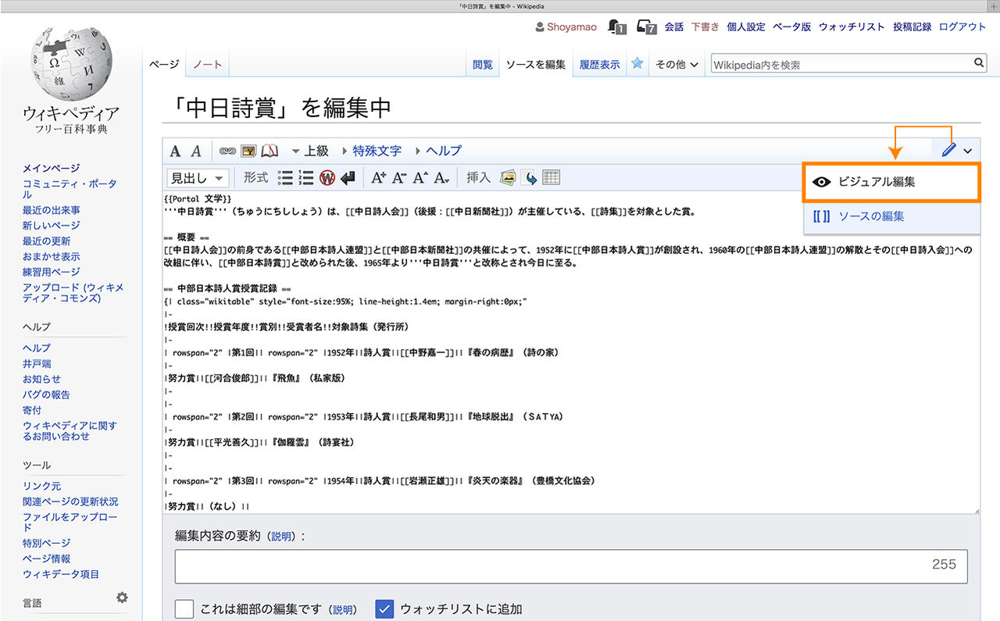
\includegraphics[width=120mm]{images/wikipedia_edit.png}
  \caption{Wikipediaでの編集画面} \label{fig:wikipedia_edit}
\end{figure}

\subsection{NFC技術とWikiの併用}
上記のようなNFC技術とWikiの利点を組み合わせることで前節の要件5も満たすことができる。

\subsubsection*{要件5:広い分野の知見と用途を総合的に管理できる}
Wikiはハイパーリンクで情報を整理・参照するため、グループによる情報分類や階層的な情報の管理を必要としない。
したがってWikiでは異なる分野の情報をフラットに管理し、参照することができる。
実際ににWikiシステムを利用した百科事典であるWikipediaはあらゆる分野の情報を総合的に管理しながらも破綻なくシステムを運用している。
このようなWikiシステムをAR情報の管理に利用することで、分野を横断した知見の管理が可能になり、様々な用途に対応したナビゲーションシステムを作成できる。

Wikiシステムを利用すると広い分野の情報を一元的に管理することができるが、一方で自身の欲しい情報を探す際に手間となる事がある。
これを避けるためにNFCタグに記録されたコンテキスト情報を活用し検索・フィルタが可能なシステムを本研究では採用した。

これより広い分野の情報を一元的に管理できるWikiの利点を活かしながら様々な用途に対応したナビゲーションを提供する事が可能となる.



\section{まとめ}
本章では第\ref{chap:background}章で整理したARナビゲーションの現状と問題点を元に次世代ARナビゲーションシステム、HypAR Touchの要件を定義した。
さらに定義した要件はNFC技術とWikiシステムを組み合わせることで達成されることを提案し、その詳細を設計で示した。
次章では本設計を元に開発したHypAR Touchの実装とその機能を説明する。